% VerdeAI gap-analysis pipeline — simplified architecture figure.
% Standalone: compiles on its own (Overleaf) to a single cropped PDF.
\documentclass[tikz, border=6mm]{standalone}
\usetikzlibrary{shapes.geometric, arrows.meta, positioning, calc}

\definecolor{inkcolor}{HTML}{17241B}
\definecolor{mutedtext}{HTML}{4D5D4F}
\definecolor{terminalfill}{HTML}{F2F3EF}
\definecolor{iofill}{HTML}{B7C6DA}
\definecolor{decisionfill}{HTML}{E6D3A3}
\definecolor{processfill}{HTML}{BFD3BC}
\definecolor{aifill}{HTML}{CBB9D6}
\definecolor{reportfill}{HTML}{3E5C43}
\definecolor{abstainfill}{HTML}{D9CBB8}

\begin{document}
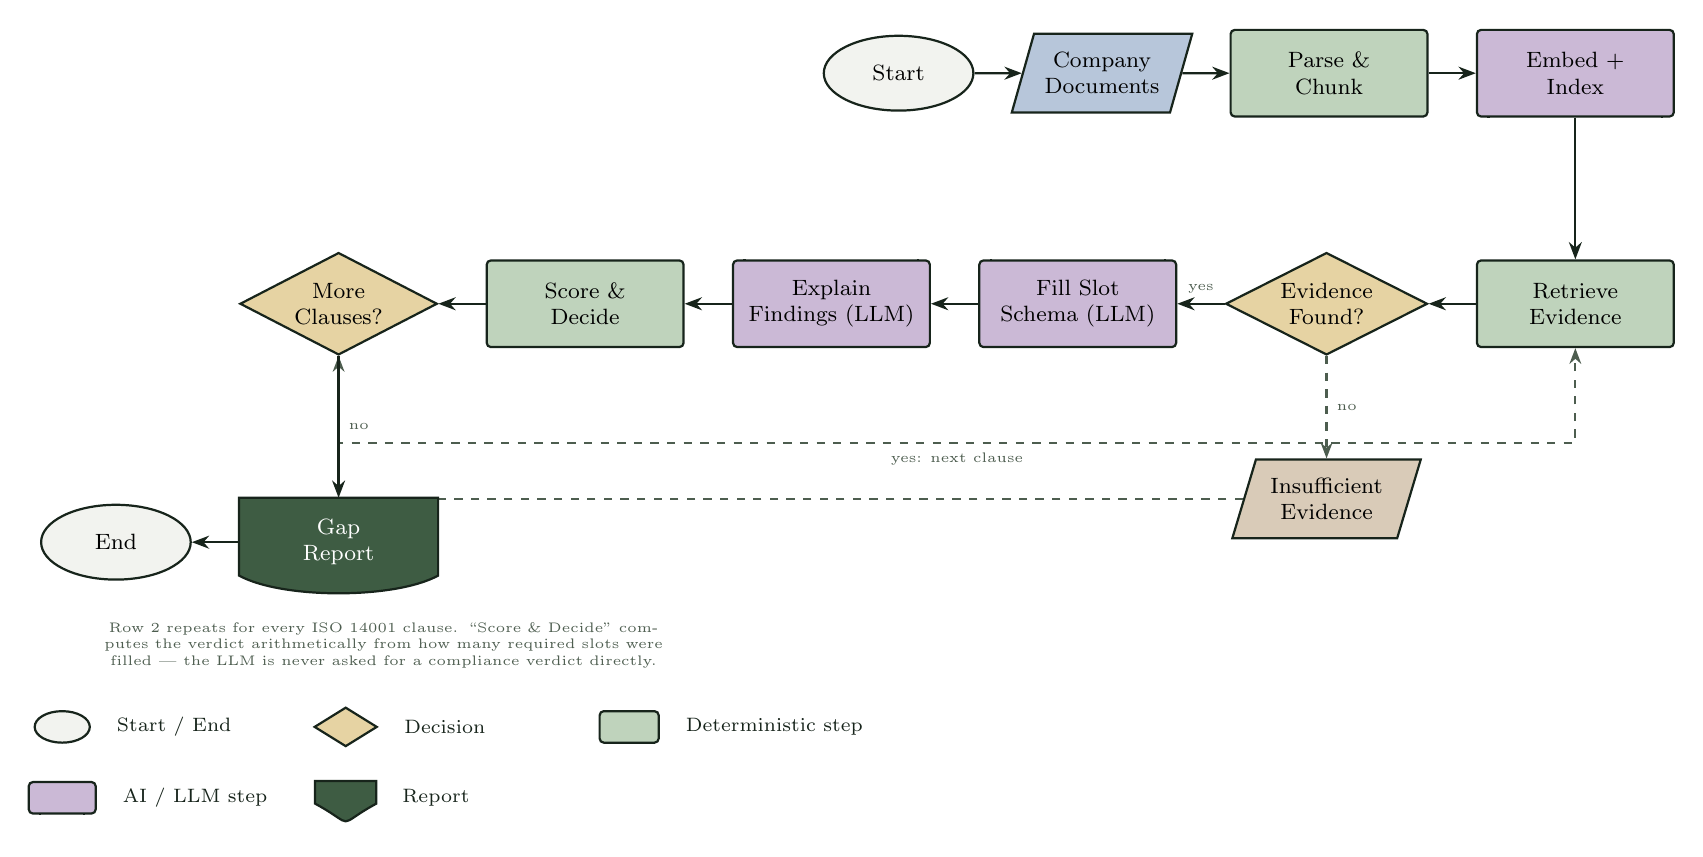
\begin{tikzpicture}[
  >=Stealth,
  every node/.style={font=\footnotesize},
  node distance=6mm and 6mm,
  align=center,
  thick,
]

\tikzset{
  terminal/.style={ellipse, draw=inkcolor, fill=terminalfill,
    minimum width=1.9cm, minimum height=0.95cm},
  io/.style={trapezium, trapezium left angle=70, trapezium right angle=110,
    trapezium stretches=true, draw=inkcolor, fill=iofill,
    minimum width=2.3cm, minimum height=1.0cm},
  abstain/.style={trapezium, trapezium left angle=70, trapezium right angle=110,
    trapezium stretches=true, draw=inkcolor, fill=abstainfill,
    minimum width=2.4cm, minimum height=1.0cm},
  decision/.style={diamond, draw=inkcolor, fill=decisionfill, aspect=2.2,
    inner sep=1pt, minimum width=2.4cm, minimum height=1.3cm},
  process/.style={rectangle, rounded corners=1.5pt, draw=inkcolor, fill=processfill,
    minimum width=2.5cm, minimum height=1.1cm},
  subprocess/.style={rectangle, rounded corners=1.5pt, draw=inkcolor, fill=aifill,
    minimum width=2.5cm, minimum height=1.1cm,
    append after command={\pgfextra{
      \draw[inkcolor] ($(\tikzlastnode.north west)!0.16cm!(\tikzlastnode.north east)$)
        -- ($(\tikzlastnode.south west)!0.16cm!(\tikzlastnode.south east)$);
      \draw[inkcolor] ($(\tikzlastnode.north east)!0.16cm!(\tikzlastnode.north west)$)
        -- ($(\tikzlastnode.south east)!0.16cm!(\tikzlastnode.south west)$);
    }}},
  flowline/.style={-{Stealth[length=2.2mm]}, inkcolor},
  branchline/.style={-{Stealth[length=2mm]}, mutedtext, dashed},
}

\newcommand{\documentshape}[2]{
  \draw[inkcolor, fill=reportfill]
    (#1.north west) -- (#1.north east)
    -- ($(#1.south east)+(0,0.14)$)
    .. controls ($(#1.south east)+(-0.55,-0.16)$) and ($(#1.south west)+(0.55,-0.16)$) ..
    ($(#1.south west)+(0,0.14)$) -- cycle;
  \node[text=white, align=center] at (#1) {#2};
}

% ---------------------------------------------------------------
% ROW 1 — ingest & index company documents (once per document)
% ---------------------------------------------------------------
\node[terminal]                     (start)   {Start};
\node[io,        right=of start]    (docs)    {Company\\Documents};
\node[process,   right=of docs]     (parse)   {Parse \&\\Chunk};
\node[subprocess,right=of parse]    (embed)   {Embed +\\Index};

% ---------------------------------------------------------------
% ROW 2 — per-clause gap analysis (repeats for every ISO clause)
% ---------------------------------------------------------------
\node[process,    below=18mm of embed]   (retrieve) {Retrieve\\Evidence};
\node[decision,   left=of retrieve]      (haseve)   {Evidence\\Found?};
\node[subprocess, left=of haseve]        (fill)     {Fill Slot\\Schema (LLM)};
\node[subprocess, left=of fill]          (analyse)  {Explain\\Findings (LLM)};
\node[process,    left=of analyse]       (score)    {Score \&\\Decide};
\node[decision,   left=of score]         (more)     {More\\Clauses?};

\node[abstain, below=13mm of haseve] (insuff) {Insufficient\\Evidence};

% ---------------------------------------------------------------
% ROW 3 — wrap up
% ---------------------------------------------------------------
\node[rectangle, minimum width=2.5cm, minimum height=1.1cm,
      below=18mm of more]           (reportbox) {};
\node[terminal,  left=of reportbox] (end)       {End};

% Main flow
\draw[flowline] (start) -- (docs);
\draw[flowline] (docs) -- (parse);
\draw[flowline] (parse) -- (embed);
\draw[flowline] (embed.south) -- (retrieve.north);
\draw[flowline] (retrieve) -- (haseve);
\draw[flowline] (haseve) -- node[above, font=\tiny, text=mutedtext]{yes} (fill);
\draw[flowline] (fill) -- (analyse);
\draw[flowline] (analyse) -- (score);
\draw[flowline] (score) -- (more);
\draw[flowline] (reportbox) -- (end);

% Branch 1 — no evidence retrieved -> abstain
\draw[branchline] (haseve.south) -- node[right, font=\tiny, text=mutedtext]{no} (insuff.north);
\draw[branchline] (insuff.west) -| node[near start, above, font=\tiny, text=mutedtext]{} (more.south);

% Branch 2 — loop back for next clause
\coordinate (loopLane) at ($(more.south)+(0,-1.1)$);
\draw[branchline] (more.south) -- (loopLane)
  -| node[near start, below, font=\tiny, text=mutedtext]{yes: next clause} (retrieve.south);

% Branch 3 — all clauses done -> report
\draw[flowline] (more.south) -- node[right, font=\tiny, text=mutedtext]{no} (reportbox.north);

\documentshape{reportbox}{Gap\\Report}

% ---------------------------------------------------------------
% Legend
% ---------------------------------------------------------------
\begin{scope}[shift={($(end.south west)+(0,-2.0)$)}]
  \node[terminal, minimum width=0.7cm, minimum height=0.4cm, font=\tiny] (l1) at (0,0) {};
  \node[right=2mm of l1, font=\scriptsize, text=inkcolor] {Start / End};

  \node[decision, minimum width=0.8cm, minimum height=0.5cm, font=\tiny] (l2) at (3.6,0) {};
  \node[right=2mm of l2, font=\scriptsize, text=inkcolor] {Decision};

  \node[process, minimum width=0.75cm, minimum height=0.4cm, font=\tiny] (l3) at (7.2,0) {};
  \node[right=2mm of l3, font=\scriptsize, text=inkcolor] {Deterministic step};

  \node[subprocess, minimum width=0.85cm, minimum height=0.4cm, font=\tiny] (l4) at (0,-0.9) {};
  \node[right=2mm of l4, font=\scriptsize, text=inkcolor] {AI / LLM step};

  \node[rectangle, minimum width=0.75cm, minimum height=0.4cm] (l5) at (3.6,-0.9) {};
  \documentshape{l5}{}
  \node[right=2mm of l5, font=\scriptsize, text=inkcolor] {Report};
\end{scope}

\node[font=\tiny, text=mutedtext, below=4mm of end, xshift=3.4cm, text width=8cm, align=center]
  {Row 2 repeats for every ISO 14001 clause. ``Score \& Decide'' computes the verdict
  arithmetically from how many required slots were filled --- the LLM is never asked
  for a compliance verdict directly.};

\end{tikzpicture}
\end{document}
